\begin{frame}
\frametitle{Ao final dessa aula, você será capaz de:}
\begin{itemize}
 \item Conhecer os principais atores/partes envolvidos em um projeto
 \item Compreender o papel do gerente de projeto em diferentes modelos organizacionais
 \item Conhecer a bibliografia/vocabulário padrão para gerenciamento de projetos
\end{itemize}
\end{frame}

\section{Organização de Projetos e Stakeholders}

\begin{frame}
   \frametitle{Organização de Projetos e Stakeholders}
   \begin{itemize}
    \item Quem vai realizar o trabalho?
    \item Quem é o Gerente de Projeto?
    \item Quem está pagando pelo projeto?
    \item Quem vai consumir o produto ou serviço?
    \item Quem são os afetados pelo projeto?
   \end{itemize}
  \end{frame}

    \begin{frame}
   \frametitle{As Partes interessadas}
   As partes interessadas no projeto (Stakeholders) são pessoas e organizações
   \begin{itemize}
    \item A relação entre as partes interessadas do Projeto:
   \end{itemize}

    \begin{figure}
  \centering
  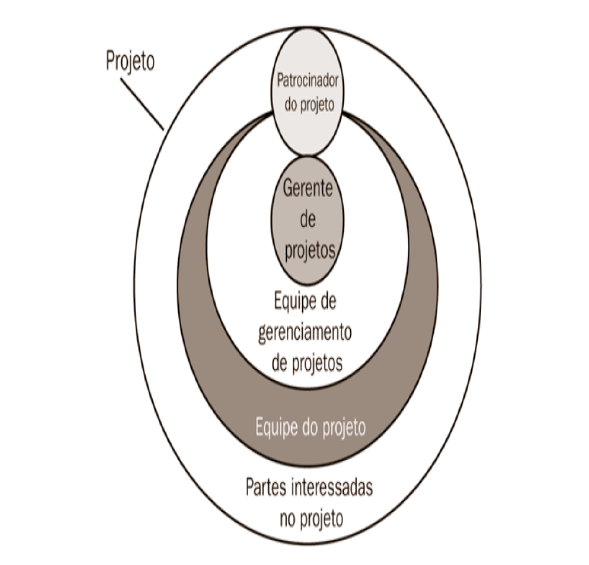
\includegraphics[width = 0.6\textwidth]{figs/fig1_2.png}
  %\caption{A relação entre as partes interessadas do Projeto}
 \end{figure}
  \end{frame}
  
  \begin{frame}
  \frametitle{Falha em comprender Stakeholders: \\
  \small{Google Wave}}
    \begin{figure}
  \centering
  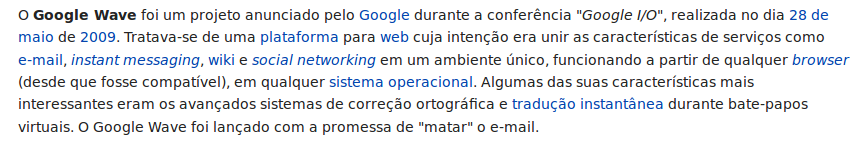
\includegraphics[width = 0.9\textwidth]{figs/fig1_7.png}
  %\caption{A relação entre as partes interessadas do Projeto}
 \end{figure}
  \begin{figure}
  \centering
  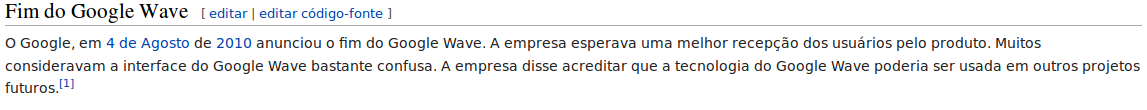
\includegraphics[width = 0.9\textwidth]{figs/fig1_8.png}
  %\caption{A relação entre as partes interessadas do Projeto}
 \end{figure}
 \footnote{Fonte:Wikipedia}
  \end{frame}

  \begin{frame}
   \frametitle{Stakeholders}
   Envolvimento dos Stakeholders com o Projeto
    \begin{figure}
  \centering
  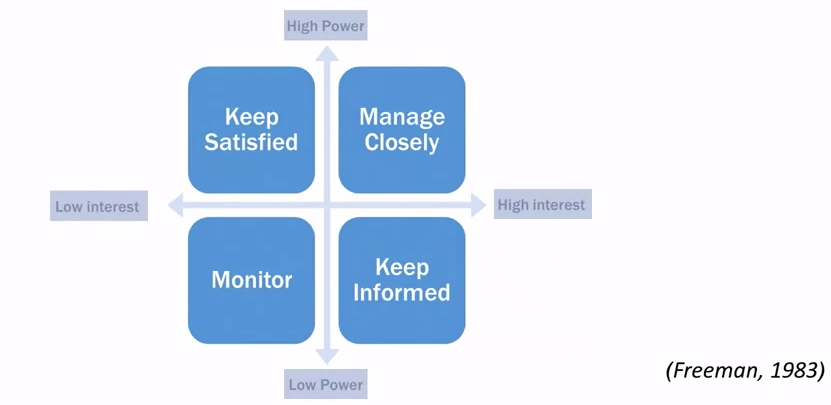
\includegraphics[width = 0.9\textwidth]{figs/fig_proj8.png}
 \end{figure}
  \end{frame}
  
\section{O papel do Gerente}
\begin{frame}
 \frametitle{O Papel}
 \begin{block}{Gerente de Projetos}
  Gerente de Projetos é CARGO? é FUNÇÃO? é HABILIDADE?
 \end{block}
 \pause
 \begin{block}{}
  Hoje, o papel de Gerente de projetos é visto como habilidade
 \end{block}
\end{frame}


  \begin{frame}
   \frametitle{O Gerente de Projetos}
   \begin{itemize}
    \item Habilidades
    \begin{itemize}
      \item Comunicação eficaz
      
     \item Motivador de pessoas
     %\pause
     \item Líder do grupo
     %\pause
     \item Organizado
     %\pause
     \item Influência sobre a organização
     %\pause
     \item Negociador
     %\pause
     \item Solucionador de problemas
     %\pause
     \item Gerenciador de Conflitos
     %\pause
     \item Facilitador entre processos
     %\pause
     \item Seguro nas decisões
    \end{itemize}
   \end{itemize}
  \end{frame}
 
\begin{frame}
 \frametitle{Necessidades Conflitantes}
 \begin{block}{Gerente de Projetos}
 Necessidades conflitantes de projetos envolvem uma “tripla restrição” – escopo, tempo e custo
 \end{block}
\end{frame}

\begin{frame}
  \begin{figure}
  \centering
  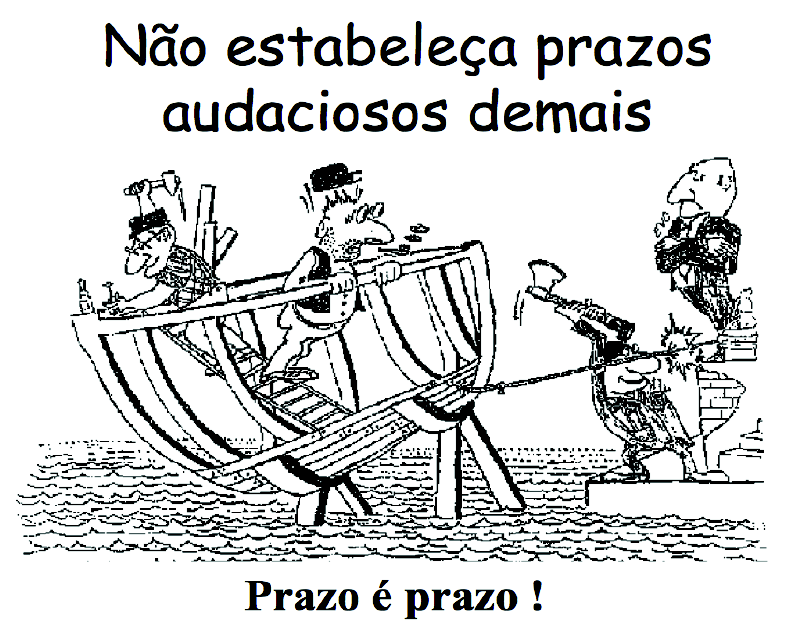
\includegraphics[width = 0.8\textwidth]{figs/fig1_1.png}
 \end{figure}
\end{frame}

\begin{frame}
   \frametitle{Contexto de GP
- Estruturas organizacionais}
   \begin{itemize}
    \item A organização \textbf{funcional clássica} é uma hierarquia em que cada funcionário possui um superior bem definido
    \begin{itemize}
     \item Os funcionários são agrupados por especialidade, como produção, marketing, engenharia e contabilidade
     %\pause
    \end{itemize}
    %\pause
    \item As organizações funcionais ainda possuem projetos, mas o escopo do projeto geralmente é restrito aos limites da função
    \begin{itemize}
     \item O departamento de engenharia em uma organização funcional fará o seu trabalho do projeto de modo independente dos departamentos de produção ou de marketing
    \end{itemize}
   \end{itemize}
  \end{frame}
  
\begin{frame}
 \frametitle{Contexto de GP - Estruturas organizacionais}
 \begin{figure}
  \centering
  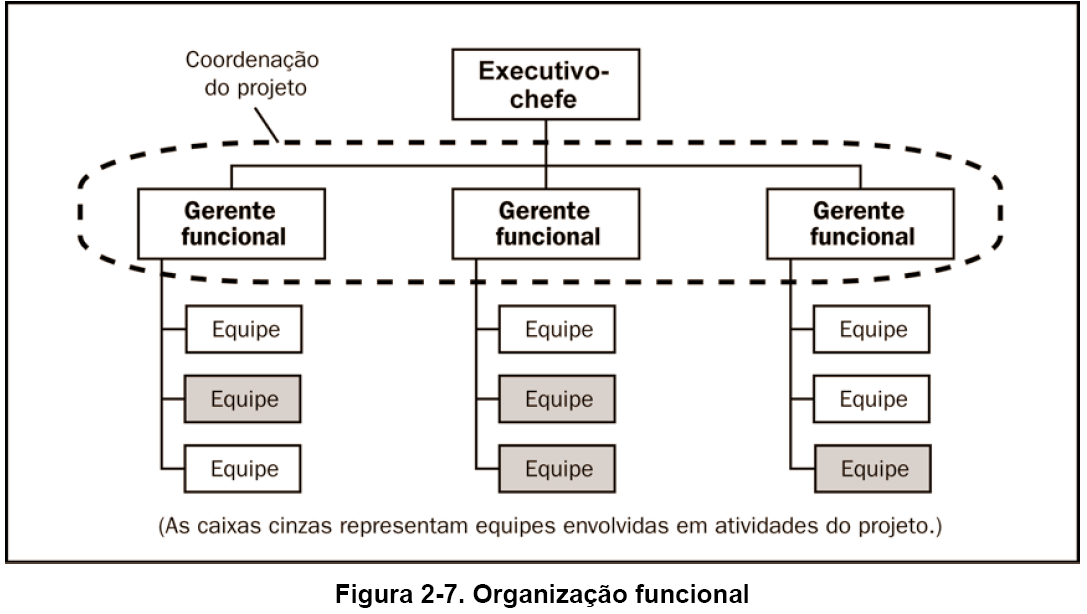
\includegraphics[width = 0.9\textwidth]{figs/fig1.png}
 \end{figure}
\end{frame}

\begin{frame}
   \frametitle{Contexto de GP
- Estruturas organizacionais}
   \begin{itemize}
    \item Em uma organização \textbf{por projeto}, os membros da equipe geralmente são colocados juntos
    %\pause
    \item A maior parte dos recursos da organização está envolvida no projeto e os gerentes de projetos possuem grande independência e autoridade
    %\pause
    \item As organizações por projeto em geral possuem unidades organizacionais denominadas departamentos, mas esses grupos se reportam diretamente ao gerente de projetos ou oferecem serviços de suporte para os diversos projetos
   \end{itemize}
  \end{frame}

  
  \begin{frame}
 \frametitle{Contexto de GP - Estruturas organizacionais}
 \begin{figure}
  \centering
  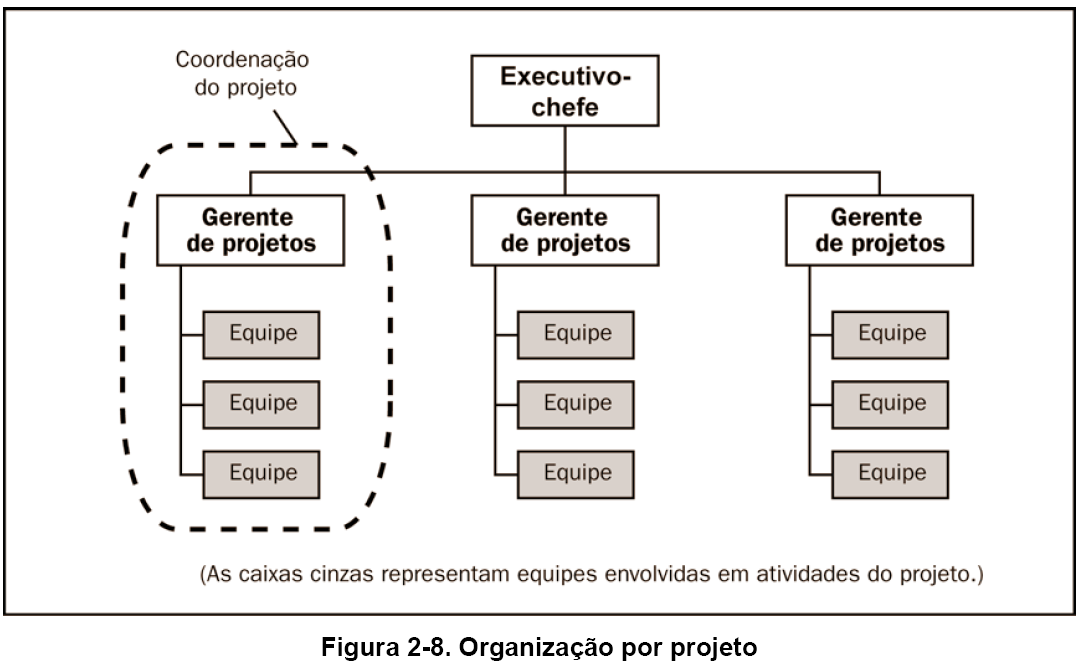
\includegraphics[width = 0.9\textwidth]{figs/fig7.png}
 \end{figure}
\end{frame}

  
  \begin{frame}
   \frametitle{Contexto de GP
- Estruturas organizacionais}
   \begin{itemize}
    \item As organizações \textbf{matriciais} são uma combinação de características das organizações funcional e por projeto
    %\pause
    \item As \textbf{matrizes fracas} mantêm muitas das características de uma organização funcional e a função do gerente de projetos é mais parecida com a de um coordenador ou facilitador que com a de um gerente
  
   \end{itemize}
  \end{frame}
  
    \begin{frame}
   \frametitle{Contexto de GP
- Estruturas organizacionais}
   \begin{itemize}
    \item Embora a organização \textbf{matricial balanceada} reconheça a necessidade de um gerente de projetos, ela não fornece ao gerente de projetos autoridade total sobre o projeto e os recursos financeiros do projeto
  %\pause
    \item As \textbf{matrizes fortes} possuem muitas das características da organização por projeto, e podem ter gerentes de projetos em tempo integral com autoridade considerável e pessoal administrativo do projeto em tempo integral. 
   \end{itemize}
  \end{frame}
  
    \begin{frame}
 \frametitle{Contexto de GP - Estruturas organizacionais}
 \begin{figure}
  \centering
  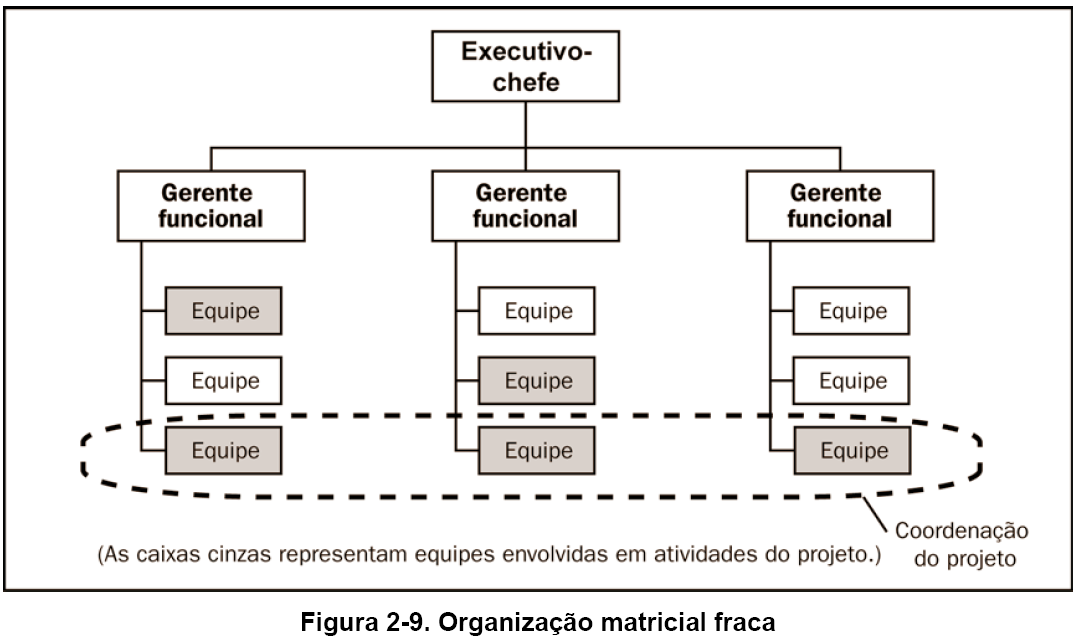
\includegraphics[width = 0.9\textwidth]{figs/fig8.png}
 \end{figure}
\end{frame}

    \begin{frame}
 \frametitle{Contexto de GP - Estruturas organizacionais}
 \begin{figure}
  \centering
  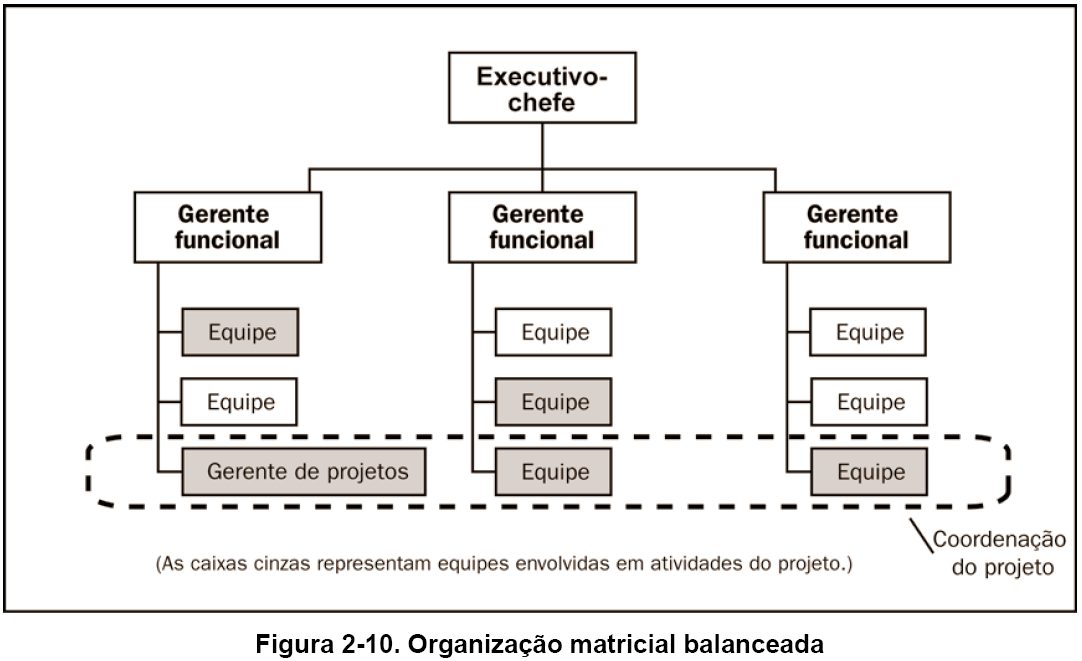
\includegraphics[width = 0.9\textwidth]{figs/fig9.png}
 \end{figure}
\end{frame}

    \begin{frame}
 \frametitle{Contexto de GP - Estruturas organizacionais}
 \begin{figure}
  \centering
  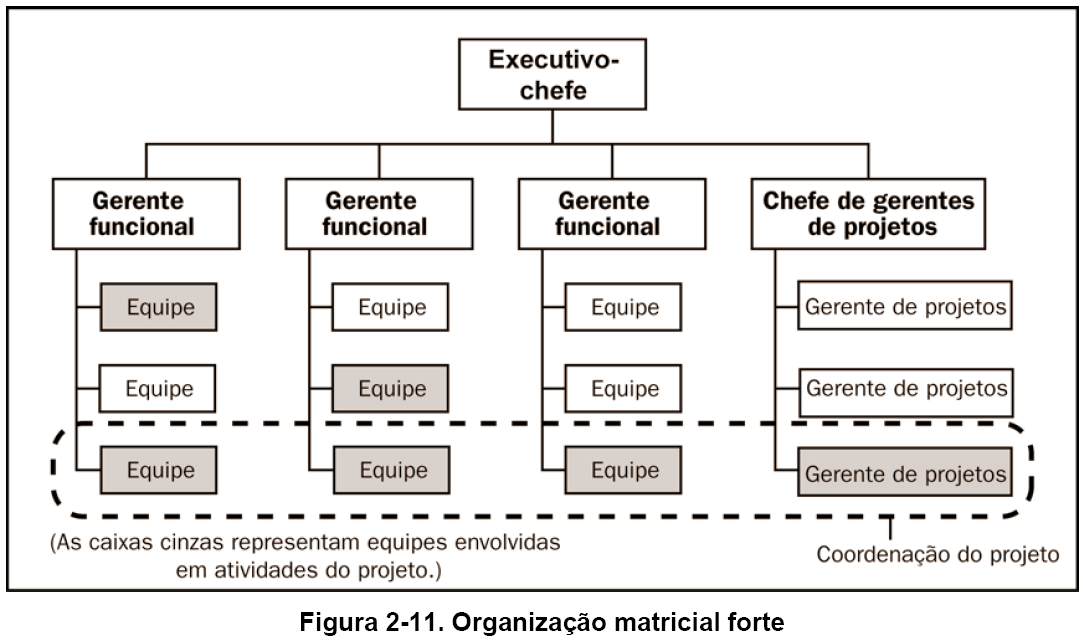
\includegraphics[width = 0.9\textwidth]{figs/fig10.png}
 \end{figure}
\end{frame}

    \begin{frame}
 \frametitle{Contexto de GP - Estruturas organizacionais}
 \begin{figure}
  \centering
  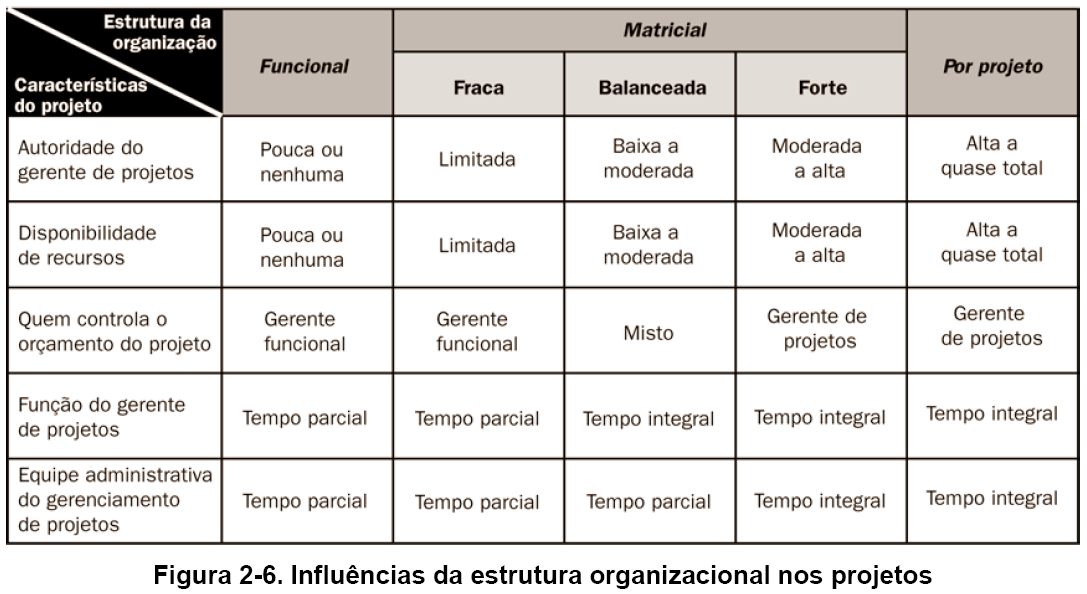
\includegraphics[width = 0.9\textwidth]{figs/fig11.png}
 \end{figure}
\end{frame}

\begin{frame}
 \begin{block}{}
  A estrutura hierárquica tradicional tipicamente atrapalha
 \end{block}
\end{frame}

\section{PMBok}
    \begin{frame}
 \frametitle{Plataforma de Gerenciamento de Projetos}
 \begin{figure}
  \centering
  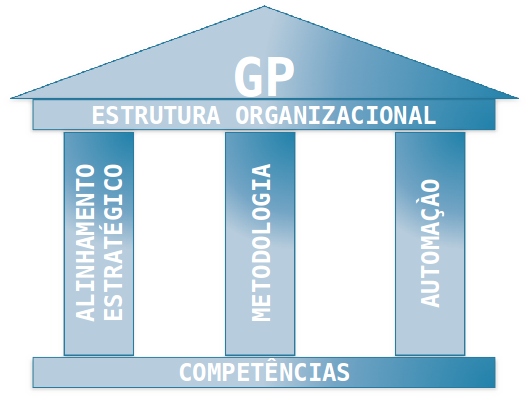
\includegraphics[width = 0.9\textwidth]{figs/fig12.png}
 \end{figure}
\end{frame}

  \begin{frame}
   \frametitle{O PMBoK}
   \begin{itemize}
    \item Guia para o Conjunto de Conhecimentos em Gerenciamento de Projetos – Guia  PMBOK®, que é mantido pelo Project Management Institute-PMI
    \begin{itemize}
     \item 1ª Edição em 1996
     %\pause
     \item 2ª Edição em 2000
     %\pause
     \item 3ª Edição em 2004
     %\pause
     \item 4ª Edição em 2008
        %\pause
     \item 5ª Edição em 2013
    \end{itemize}
  \item Uma norma Nacional Americana (ANSI)
   \end{itemize}
  \end{frame}
  
    \begin{frame}
   \frametitle{Sobre o PMBoK}
   \begin{itemize}
    \item Identificar o subconjunto do conjunto de conhecimentos em gerenciamento de projetos que é amplamente reconhecido como boa prática
    \begin{itemize}
     \item Visão geral, não uma descrição completa
     %\pause
     \item Conhecimento e práticas descritas são aplicáveis à maioria dos projetos na maior parte do tempo
     %\pause
     \item A aplicação correta dessas habilidades, ferramentas e técnicas podem aumentar as chances de sucesso
    \end{itemize}
    %\pause
    \item Uma boa prática não significa que o conhecimento descrito deverá ser sempre aplicado uniformemente em todos os projetos
    \begin{itemize}
     \item A equipe de gerenciamento de projetos é responsável por determinar o que é adequado para um projeto específico
    \end{itemize}
   \end{itemize}
  \end{frame} 	
  
      \begin{frame}
   \frametitle{Sobre o PMBoK}
   \begin{itemize}
    \item O conhecimento descrito no PMBOK consiste em
    \begin{itemize}
     \item Definição do ciclo de vida do projeto
     %\pause
     \item Cinco grupos de processos
     %\pause
     \item Nove áreas de conhecimento
    \end{itemize}
   \end{itemize}
  \end{frame}
  
        \begin{frame}
 \frametitle{PMBok - Áreas de  Conhecimento}
 \begin{figure}
  \centering
  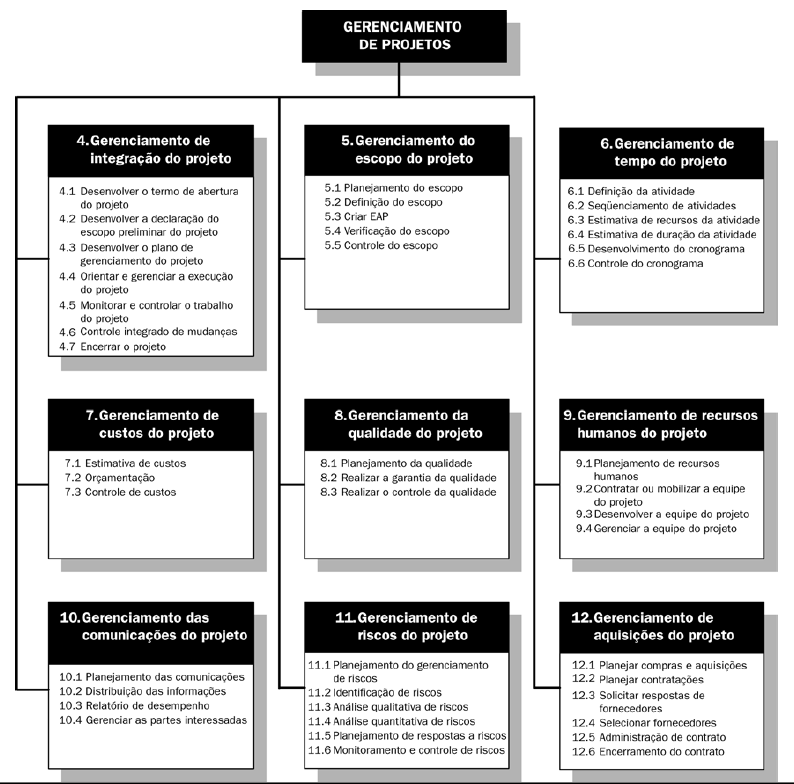
\includegraphics[height = \textheight]{figs/fig_proj7.png}
 \end{figure}
\end{frame}

      \begin{frame}
 \frametitle{PMBok - Áreas de  Conhecimento}
 \begin{figure}
  \centering
  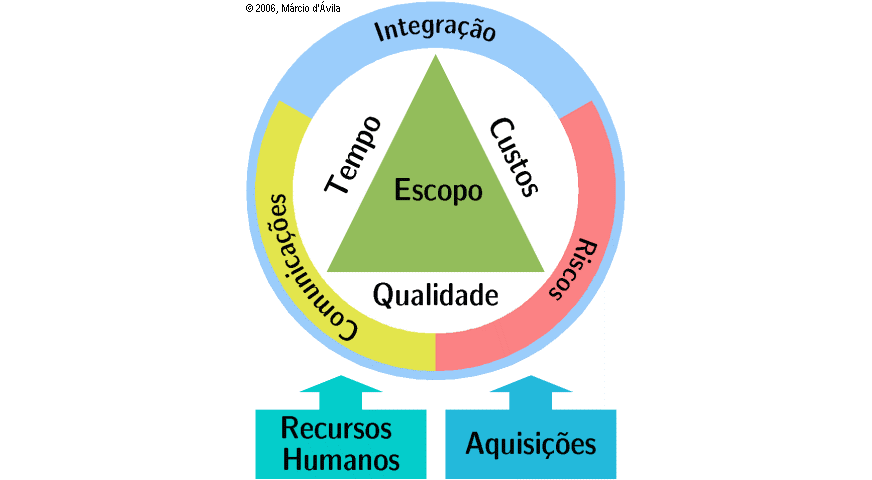
\includegraphics[width = \textwidth]{figs/fig13.png}
 \end{figure}
\end{frame}




\begin{frame}
 \frametitle{Visão Geral dos Processos de Gerenciamento de Projetos}
 \begin{figure}
  \centering
  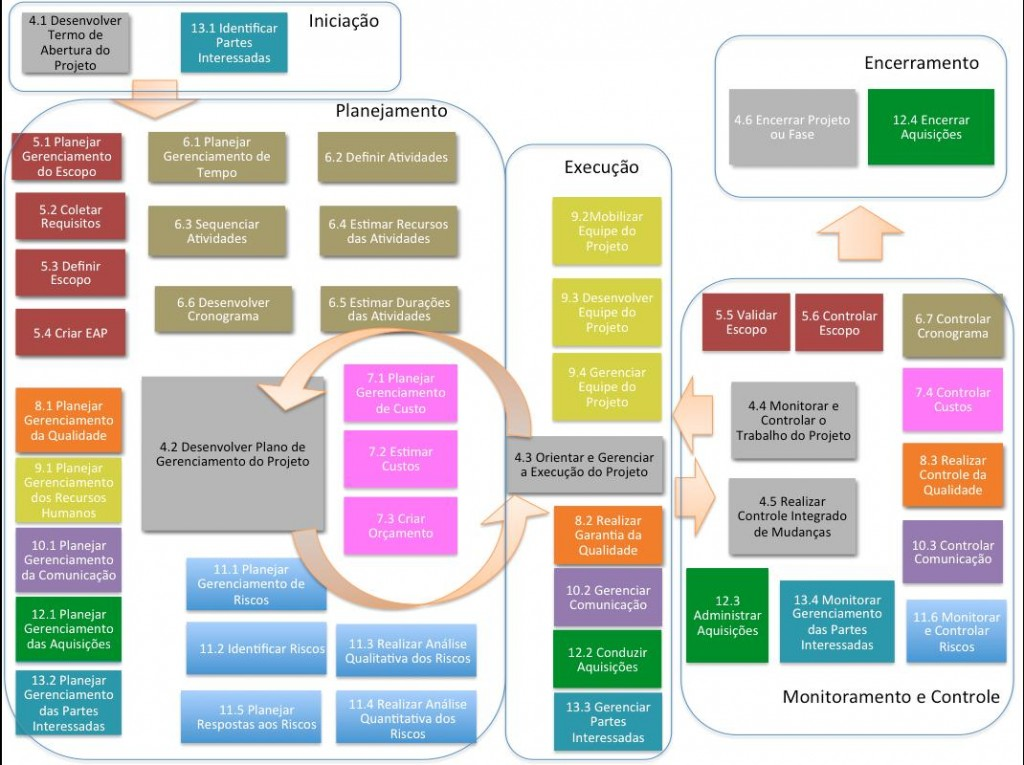
\includegraphics[width = \textwidth]{figs/figura-4-1024x765.jpg}
 \end{figure}
\end{frame}
\section{Método Ágil}
\begin{frame}
 \frametitle{Scrum - Um método Ágil}
 \begin{block}{Definição Informal}
Estratégia em um jogo de rugby onde
jogadores colocam uma bola quase perdida
novamente em jogo através de trabalho em
equipe.
 \end{block}
 \begin{figure}
  \centering
  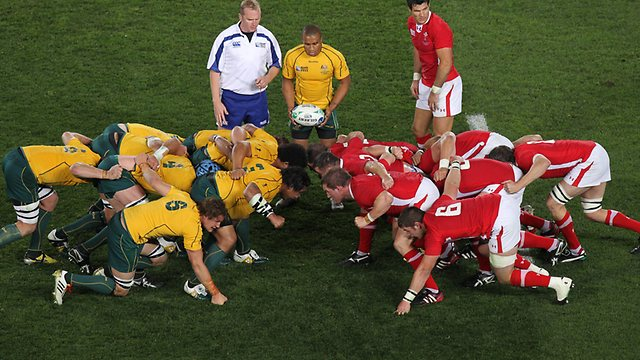
\includegraphics[width = 0.5\textwidth]{figs/326341-wallabies-scrum.jpg}
 \end{figure}
\end{frame}

\begin{frame}
 \frametitle{O manifesto do \\
 \small{Desenvolvimento Ágil de Software}}
 \begin{itemize}
  \item \textbf{Indivíduos e interações} são mais importantes que processos e ferramentas
  \item \textbf{Software Funcionando} é mais importante que documentação completa e detalhada
  \item \textbf{Colaboração com o cliente} é mais importante que negociação de contratos 
  \item \textbf{Adaptação a mudança} é mais importante do que seguir o plano inicial
 \end{itemize}
\end{frame}

\begin{frame}
 \frametitle{Princípios do Manifesto Ágil}
 \begin{itemize}
  \item \textbf{Objetivo}: satisfazer o cliente entregando, rapidamente e com frequência, sistemas de algum valor, sistemas rodando em produção
  \begin{itemize}
   \item Entregar versões  funcionais em curto prazo
   \item Mudanças são um aspecto intrínsico da vida do software
   \item Software evolui para atender o negócio (união dos mundos)
   \item Troca de informações através de conversas diretas
  \end{itemize}
 \end{itemize}
\end{frame}

\begin{frame}
 \frametitle{Características Scrum}
 \begin{itemize}
  \item Equipes que se auto-organizam
  \item O produto evolui em uma espécie  de "Sprints" mensais
  \item Os requisitos sao listados em um "Product Backlog"
  \item Usa regras generativas na criação de um ambiente ágil para entrega de projetos
  \item É uma das metodologias ágeis
 \end{itemize}
\end{frame}

\begin{frame}
 \frametitle{Scrum - Fases}
 \begin{figure}
  \centering
  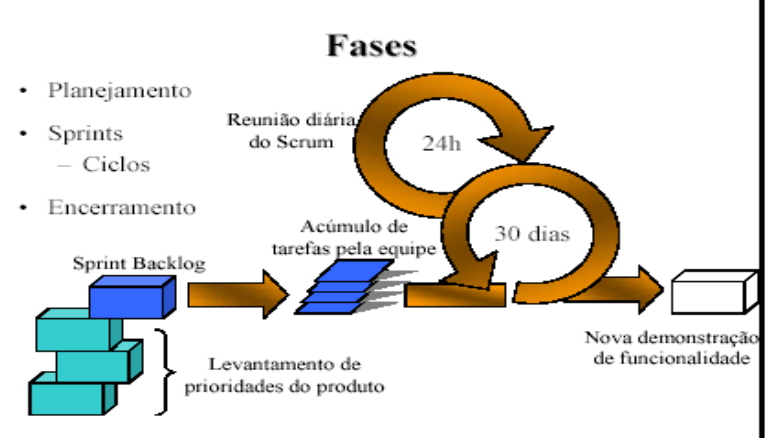
\includegraphics[width = 0.7\textwidth]{figs/fig1_5.png}
 \end{figure}
\end{frame}

\begin{frame}
 \frametitle{Scrum - Planejamento do Sprint}
 \begin{figure}
  \centering
  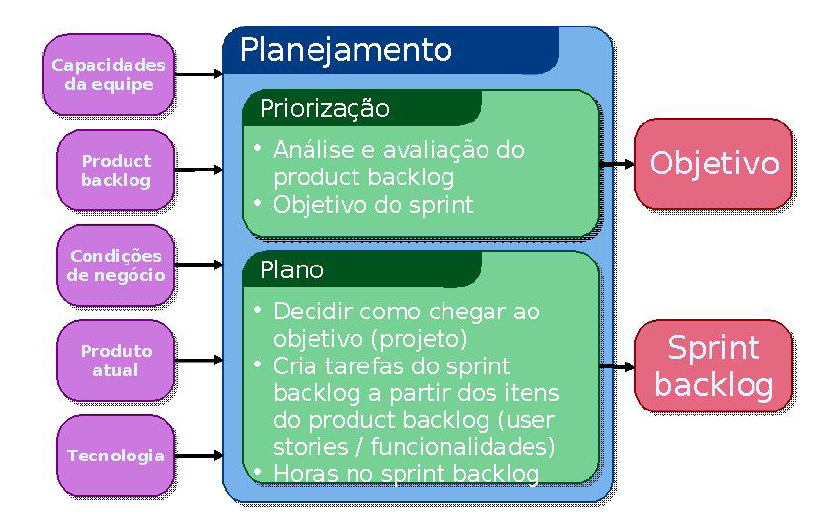
\includegraphics[width = 0.7\textwidth]{figs/fig1_6.png}
 \end{figure}
\end{frame}

\begin{frame}
 \frametitle{Scrum Diário}
 \begin{itemize}
  \item Parâmetros
  \begin{itemize}
   \item Diário
   \item 15 minutos
  \end{itemize}
  \item Todos de Pé
  \item Não é para solução de problemas
  \item Ajuda a evitar reuniões adicionais desnecessárias
 \end{itemize}
\end{frame}

\begin{frame}
 \frametitle{Reflexões na Daily-meeting}
 \begin{itemize}
  \item O que fizemos de bom e de ruim?
  \item Quais são nossas prioridades?
  \item O que mantivemos de mais importante?
  \item O que podemos mudar para a próxima vez?
  \item O que podemos adicionar/tirar?

  \item Após 2 ou 3 sprints, a metodologia deve começar a convergir para uma metodologia tolerável para o projeto
 \end{itemize}
\end{frame}

\begin{frame}
 \frametitle{Gerenciando o Sprint Backlog}
 \begin{itemize}
  \item Cada indivíduo escolhe o trabalho que fará
  \begin{itemize}
   \item Trabalhos nunca são atribuidos
  \end{itemize}
  \item Atualização diária da estimativa do trabalho restante
  \item Qualquer membro da equipe pode adicionar, apagar ou mudar tarefas
  \item O trabalho aparece a partir da Sprint
  \item Se uma tarefa não é clara, defina-a como um item com uma quantidade maior de tempo e subdivida-a depois
  \item Atualize as coisas a serem feitas na medida em que se tornam mais conhecidas
 \end{itemize}

\end{frame}

\section{Bibliografia}
\begin{frame}
 \frametitle{Bibliografia da Aula - Leitura sugerida}
 \begin{itemize}
  \item \textit{Um guia do Conjunto de Conhecimentos em Gerenciamento de Projetos - guia PMBOK} (Cap. 1)
  \item \textit{Fundamentals of Project Planning and Management} - coursera (week 1) - \url{https://class.coursera.org/projects101-002/wiki/resources}
  \item \url{https://hbr.org/1998/03/bringing-discipline-to-project-management}
  \end{itemize}

\end{frame}
